% Chapter Template

\chapter{Introduction} % Main chapter title

\label{Chapter1} % Change X to a consecutive number; for referencing this chapter elsewhere, use \ref{ChapterX}
%----------------------------------------------------------------------------------------

% Define some commands to keep the formatting separated from the content 
\newcommand{\keyword}[1]{\textbf{#1}}
\newcommand{\tabhead}[1]{\textbf{#1}}
\newcommand{\code}[1]{\texttt{#1}}
\newcommand{\file}[1]{\texttt{\bfseries#1}}
\newcommand{\option}[1]{\texttt{\itshape#1}}

%----------------------------------------------------------------------------------------
%	SECTION 1
%----------------------------------------------------------------------------------------

reasoning:
https://www.unwater.org/our-work/integrated-monitoring-initiative-sdg-6

"Stronger accountability: Data can communicate that work is being done and progress is happening. Data can enable greater transparency, which reduces inefficiency and corruption.
Attracting commitment and investments: Data can quantify problems and make it easier to communicate needs for political commitment and public and private investments.
Evidence-based decision-making: Data can inform policy- and decision-makers of where to focus efforts and which solutions are most effective, to ensure the greatest possible gains with existing resources.
Leaving no one behind: Disaggregated data can help identify specific groups or areas with unmet needs and higher levels of risk, to which interventions can be targeted."
https://www.unwater.org/our-work/integrated-monitoring-initiative-sdg-6/background

“Experts in trigger methodology have indicated a more appropriate strategy may be to build on tools that currently exist at the government level such as national drought monitoring systems. As such, the ideal is an iterative process with the ground level along with a technology push that creates new ways to analyse drought and drought risk.” ([RCRC, 2020, p. 28](zotero://select/groups/4773535/items/UESIQTRJ)) ([pdf](zotero://open-pdf/groups/4773535/items/P5JPVZ97?page=28&annotation=977VS8FC))

% --> even the RCRC is still looking for good triggers -> maybe water levels are a good way -> reasoning for this study (see background identical text)

“Countries in which less than 50\% of the population uses improved drinking water sources are all located in sub-Saharan Africa and Oceania 91-100\% 76-90\% 50-75\% <50\% insufficient data or not applicable Proportion of the population using improved drinking water sources in 2015 ■ 91–100\% ■ 76–90\% ■ 50–75\% ■ <50\% ■ INSUFFICIENT DATA OR NOT APPLICABLE” ([World Health Organization, 2016, p. 15](zotero://select/groups/4773535/items/KVAKZ9ZT)) ([pdf](zotero://open-pdf/groups/4773535/items/4STYK52H?page=14\&annotation=FBURDS4T))

“The methods by which the Joint Monitoring Programme (JMP) of WHO and UNICEF” ([Bartram et al., 2014, p. 8137](zotero://select/groups/4773535/items/6AWUJTW5)) ([pdf](zotero://open-pdf/groups/4773535/items/BFNSQGWS?page=1&annotation=UL4Q2I4V))
“substantial limitations: current methods do not address water quality, equity of access, or extra-household services.” ([Bartram et al., 2014, p. 8137](zotero://select/groups/4773535/items/6AWUJTW5)) ([pdf](zotero://open-pdf/groups/4773535/items/BFNSQGWS?page=1&annotation=TIPCEXGG))



what drought is (definition)
drought monitoring but not only physical indicators but socials as well (water source accessibility) “However, assessments focused only on physical variables and processes fail to capture why drought matters, in other words, how social, economic, and ecological systems are affected (i.e., impacts) (Redmond 2002; Van Loon et al. 2016; Wilhite and Glantz 1985).” ([Lackstrom et al., 2022, p. 3](zotero://select/groups/4773535/items/YI366LQY)) ([pdf](zotero://open-pdf/groups/4773535/items/3JTQ72UN?page=3\&annotation=72WYIE7B))
current monitoring approaches e.g. (“the extent to which volunteers’ assessments of dry-to-wet conditions correspond to objective drought indicators (EDDI, SPI, SPEI) typically employed for monitoring drought” ([Lackstrom et al., 2022, p. 2](zotero://select/groups/4773535/items/YI366LQY)) ([pdf](zotero://open-pdf/groups/4773535/items/3JTQ72UN?page=2\&annotation=DQ4ZNIRS)))
“quantitative indicators (namely the SPEI, SPI, and EDDI).” ([Lackstrom et al., 2022, p. 26](zotero://select/groups/4773535/items/YI366LQY)) ([pdf](zotero://open-pdf/groups/4773535/items/3JTQ72UN?page=26\&annotation=G4KIJYUR))

which forecasts are selected by the EAP pre-study?
request of the SRCS -> practically wanted
understanding the full scope and knowing which water sources are at what level and quality can help with management decisions and trigger certain events very locally
current challenges (?) what do I want to address? (number 1,2,3)
outline of the thesis/project

what about the volunteers? how many? where are they? How to they spread over the country?
“Meadow et al. (2013) recommended using trained agency staff to report drought status on a regular basis” ([Lackstrom et al., 2022, p. 27](zotero://select/groups/4773535/items/YI366LQY)) ([pdf](zotero://open-pdf/groups/4773535/items/3JTQ72UN?page=27\&annotation=AUZV7SZN))

overcome limitations / incorporating recommendations: e.g. increased support/engagement of poeple who actually use the reports (e.g. SRCS officials) 
fill geographic and information gap ->

its about drought forecasting and early trigger but at the same time highly local and practical information where and which water sources are good and functioning and which are not. -> highly practical information. Some data exist but (mostly) outdated.
about getting local knowledge from SRCS Volunteers and their community as well as returning information about the bigger picture
in order to enhance the quality of data for managing severe droughts in Somaliland. (one short paragraph -> motivation)
provide number of weather stations in the area

relevance
Somalia is komplett am krepieren because of a multi-year long drought - ...\% of damage/conflicts etc. is based on droughts. severe shit! --> first case study introduction (geographically, socially, etc.) 
scope: of the EAP/FbF project

--> FbF and EAP what is what and so on --> in context of this work -> drought indicator (what exists so far? -> pre study)
Somalia red Crescent Society scope etc. 

--> problem: conclusion of existing sources, tools and forecasts - only macro/international level? or are there meso/micro forecasts available?
better understanding the forecasting and its implications on the ground are crucial. --> local information. tons of Volunteers but even more water sources. Continue with Crowdsensing? Implications?

--> highlight the pro of this work
"The highly localized information provided by observers can fill drought monitoring gaps by ground-truthing quantitative indicators and offering information in places where other monitoring tools may not exist. Overall, the research team found that strategic investments in time and funding can help fill in geographic and temporal gaps in drought monitoring information through volunteer observations."
https://www.drought.gov/news/research-confirms-role-citizen-science-contributions-drought-detection-and-monitoring and https://doi.org/10.1175/BAMS-D-21-0157.1


“Citizen science programmes are promising cost-efficient methods to monitor environmental resources, which make them especially suitable for low-income countries to overcome their sparse data resolution.” ([Weeser et al., 2018, p. 1598](zotero://select/groups/4773535/items/SFA2MLHC)) ([pdf](zotero://open-pdf/groups/4773535/items/GP79FHFC?page=9&annotation=4E9JCTQ5))
“Since today's citizen science studies are mostly located in high-income countries, we are enthusiastic to motivate the scientific community to conduct citizen science studies in low-income countries.” ([Weeser et al., 2018, p. 1598](zotero://select/groups/4773535/items/SFA2MLHC)) ([pdf](zotero://open-pdf/groups/4773535/items/GP79FHFC?page=9&annotation=TYD7Q2ZD))


key aims and objectives + research questions

incorporating local knowledge? - if yes, how?
how to account for gender inequalities? Even possible?

current challenges for utilisation of forecasting systems: scarse coverage of weather stations and poor utilisation by the farmers often due to bad dissemination channels  (too coarse, too unreliable)

provide hypothesis - 'integration' of local stakeholders/volunteers into drought and water source monitoring can help to get a better picture for early drought impact assessment and thus better and faster management and reactions
+ local people are engaged with the process and come into contact with 'scientific' knowledge/forecasts 
+ equal inclusion of local / indigenous knowledge and scientific forecasts can enhance the quality and make it more relevant on smaller scales (meso/mikro/local level)


how it was done: methods are qualitative, half-structured interviews, literature review and conceptualizing a tool based on current best practices

outline structure

knowledge co-production
\autocite{dasInteractiveInformationCrowdsourcing2016}

conceptualization: evtl. den 4er Zirkel?

bridge theory and practice
%-----------------------------------
%	SUBSECTION 1
%-----------------------------------
\section{Section 1}
Definitions of terminology
drought
local knowledge
\subsection{Subsection 1}


%-----------------------------------
%	SUBSECTION 2
%-----------------------------------

\subsection{Subsection 2}
benefits of monitoring by external support:
“Therefore, the model of community management combined with external support has far-reaching benefits to rural water supply.” ([Huang et al., 2020, p. 144](zotero://select/groups/4773535/items/9CSBLJNJ)) ([pdf](zotero://open-pdf/groups/4773535/items/G5BEZQ7C?page=9&annotation=HU2CNZC2))

“For local communities, their needs of safe drinking water could be met and their abilities to manage and maintain water supply could be enhanced.” ([Huang et al., 2020, p. 144](zotero://select/groups/4773535/items/9CSBLJNJ)) ([pdf](zotero://open-pdf/groups/4773535/items/G5BEZQ7C?page=9&annotation=AL2NB5DK))

“For external experts, they may also benefit from community support to inform scientific processes, such as collecting data that spans across a large geographic region and having an enhanced understanding of community interests.” ([Huang et al., 2020, p. 144](zotero://select/groups/4773535/items/9CSBLJNJ)) ([pdf](zotero://open-pdf/groups/4773535/items/G5BEZQ7C?page=9&annotation=QPIKDKB9))

“Furthermore, this model could help increase scientific awareness among community members and engage the community with the environment.” ([Huang et al., 2020, p. 144](zotero://select/groups/4773535/items/9CSBLJNJ)) ([pdf](zotero://open-pdf/groups/4773535/items/G5BEZQ7C?page=9&annotation=FYU4BIKP))

“During the management of rural drinking water sources, a hybrid modality in which community management is the mainstay with supplement from external support from other organizations is highly recommended.” ([Huang et al., 2020, p. 147](zotero://select/groups/4773535/items/9CSBLJNJ)) ([pdf](zotero://open-pdf/groups/4773535/items/G5BEZQ7C?page=12&annotation=SQ6P8UBN))

“Community cultures, economies, and environments differ across countries and regions. These differences should be considered when designing hybrid management strategies, so that all actors can be appropriately enabled and the mechanism which is most effective for the given community can be identified.” ([Huang et al., 2020, p. 147](zotero://select/groups/4773535/items/9CSBLJNJ)) ([pdf](zotero://open-pdf/groups/4773535/items/G5BEZQ7C?page=12&annotation=WV5DXV5I))

“On this basis, it is essential to expand research area to study the various threats from climate variability to rural drinking water safety, and then to develop corresponding measures to address those threats to water security.” ([Huang et al., 2020, p. 147](zotero://select/groups/4773535/items/9CSBLJNJ)) ([pdf](zotero://open-pdf/groups/4773535/items/G5BEZQ7C?page=12&annotation=HCQHR7YR))
%----------------------------------------------------------------------------------------
%	SECTION 2
%----------------------------------------------------------------------------------------

\section{Main Section 2}

10\% (8 pages)

establish your research territory: general information about the importance, background details to understand studies context
justifying your niche - why the research is needed. -> how Gap
explain the significance of your study -> how the research was conducted -> value of the study

---
what is the topic of your thesis?
what are the objectives
what is the outline
methods?
thesis statement

Introduce the topic of the study.
Provide some general background info about your study.
Give a short overview of the literature review (we use the word short because the main lit review will be in Chapter Two: Literature Review.
Bring out the general idea of the study or the scope.
Provide the details of the current situation about the problem.
Describe the relevance of the research that you are going to present (note that you are introducing a study that you have already completed).
Outline the key aims and objectives of the dissertation.
Bring out the research questions or problems of the study.
Provide your hypothesis.
Outline the structure of your dissertation.
Highlight the methodology that you used to do the study.


acknowledge former studies
structure 
surprise (gender and the role of "integration")
best examples and best literature review
write a draft

Motivation of the study.
Description of the study topic.
Explanation of the relevance of the study.
Explanation of the scope of the study.
Demonstration of how the study was done.
Your dissertation outline.



% Chapter Template

\chapter{Proposal} % Main chapter title

\label{Proposal} % Change X to a consecutive number; for referencing this chapter elsewhere, use \ref{ChapterX}
%----------------------------------------------------------------------------------------

% Define some commands to keep the formatting separated from the content 
\newcommand{\keyword}[1]{\textbf{\#1}}
\newcommand{\tabhead}[1]{\textbf{\#1}}
\newcommand{\code}[1]{\texttt{\#1}}
\newcommand{\file}[1]{\texttt{\bfseries\#1}}
\newcommand{\option}[1]{\texttt{\itshape\#1}}

%----------------------------------------------------------------------------------------
%	SECTION 1
%----------------------------------------------------------------------------------------

\section{Introduction}
\# Overview
\#\# Motivation: Importance of Drought + local users

With the projection of rising frequency and intensity of droughts throughout vast parts of the African continent, measures for prediction, monitoring and evidence based anticipatory actions and management become ever more important \autocite{abdulkadirAssessmentDroughtRecurrence2017,adelekanAfricaClimateChange2022,vereintenationenSpecialReportDrought2021}.

In order to meet this challenge, the Red Cross Red Crescent Movement together with the Red Cross Red Crescent Climate Center started the Forecast-based Financing (FbF) programme in 2007 to facilitate Anticipatory Actions instead of post-disaster reactions. Together with their local partners, the International Federation of Red Cross Red Crescent Societies (IFRC) is working on establishing so called Early Action Protocols (EAPs) to ensure better organization and coordination of Anticipatory Actions in the face of an incoming hazard. These actions are based on a predefined interplay of forecast, trigger and financing mechanisms to ensure rapid, scientific based responses.

Somaliland, being no exception to the above mentioned climatic trend, is characterized by droughts with far reaching impacts on ecological, economic, and social aspects. Defined by a semi-arid, four-season climate with two extensive dry seasons and an economic backbone of pastoralism and rain-fed agriculture, water accessibility is of key importance in Somaliland \autocite{abdulkadirAssessmentDroughtRecurrence2017,petrucciLandscapeLandformsNorthern2022,republicofsomalilandSomalilandCountryProfile2021}.
In addition, the final report of the FbF feasibility study identifies five other hazards besides droughts, namely flood, cyclone, disease, locusts and conflict. Of all these hazards, drought was ranked as the greatest threat due to its increasing frequency, severity and wide-ranging consequences.\newline

Existing drought forecasts and trigger indicators are mostly based on physical indicators and cover especially macro- and international levels, e.g. EDDI, SPI, SPEI \todo{look them up + which forecast is defined by the SRCS?}. Fine grained up-to-date forecasts which not only include physical but also social circumstances and knowledge on local levels are often scarce or even non-existent \todo[fancyline]{sources}. "However, assessments focused only on physical variables and processes fail to capture why drought matters [...]."\autocite[3]{lackstromBackyardHydroclimatologyCitizen2022}, how it impacts communities and which mitigation strategies are locally taken \todo{source?}.\newline

Besides the further development of more fine grained technical solutions the integration of local knowledge is another way forward. Engaging local people and communities and giving them an active voice in defining and co-producing anticipatory actions and knowledge can be of multiple benefit to communities and enrich the data generated \autocite{somaliredcrescentsocietyFeasibilityStudyPotential2022, njambi-szlapkaIntegratingCommunityVoices}\todo{source}. On the one hand, citizens can help to fill data gaps of categorized measurements such as simple assessments of dry-to-wet conditions which correspond to the above mentioned technical drought indicators \autocite{lackstromBackyardHydroclimatologyCitizen2022}. On the other hand, citizens can contribute their local knowledge which can potentially draw on years of experience, encompass a wide range of aspects and give them a feeling of co-owning which in itself can already bring many advantages \autocite{njambi-szlapkaIntegratingCommunityVoices}\todo{source}. The IFRC states, that the "community engagement and accountability (CEA) is essential […] to build acceptance and trust” \autocite{ifrcCommunityEngagementAccountability}(IFRC n.d.) for effective and sustainable outcomes. 
Nonetheless, direct contributions and communication from and with volunteers or community members remain a challenge in the joint management of hazards and risks. The tasks are numerous and need to take into consideration different aspects, ranging from cultural differences to different background knowledge and technical capabilities and capacities.

Qualitative interviews can capture a wide range of local contribution, knowledge and information but are very labour intensive, often limited in time and hence not feasible on larger scale for monitoring purposes. Providing a technical solution that enables mutual contact between communities and the Somalia Red Crescent Society (SRCS) in a simple and accessible way would make it possible to collect this most helpful information. By ensuring that sovereignty over the collected data rests with the community, the decision-making power and benefits remain with those concerned. Therefore, in the development and application of an Early Action Protocol (EAP) in the context of Forecast based Action (FbA) in Somalia, the technical aspect in particular holds great potential to benefit numerous communities over the long term.

While there is a comparatively good basis with regard to the general availability of data on social, economic and natural information and conditions, as well as their spatial and qualitative characteristics, the timeliness of this information varies greatly. Especially in the context of Anticipatory Action, time is of the essence and a swift action based on up-to-date data is crucial. Gathering and incorporating local knowledge through manual surveys by a central organisation can be of great value, as shown above, but is time-consuming and slow.

The benefits of overcoming the high labour costs and the temporal handicap by providing a simple and accessible tool for the SRCS’s large network of volunteers can already be seen in other comparable contexts using the Community Based Surveillance (CBS) programme, its successor NYSS, the Ushahidi platform or tools like Social.Water, ITIKI and CoCoRaHS \autocite{fienenSocialWaterCrowdsourcing2012a} \todo{sources}. The CBS is a pioneering technical approach to disease outbreak surveillance in Somalia and was developed as part of the SRCS Health Strategy 2019-2023. In this process, “volunteers report health risks through their respective locations and send to the SRCS data platform […]” \autocite[57]{somaliredcrescentsocietyFeasibilityStudyPotential2022} through coded SMS. So far, 315 volunteers from 115 villages have specifically been trained. In at least two cases, an outbreak could be contained thanks to early detection (SRCS 2021, 2022). On top of this already proven application, further functions could be added as needed.
Social.Water, ITIKI and CoCoRaHS are environmental data collection and drought monitoring implementations. These approaches are based on Crowdsensing approaches and partly employ more sophisticated technical solutions via internet connections, wireless sensor networks or photographs and have been implemented and tested in recent studies or ongoing monitoring programmes. While suggesting that the method of Crowdsensing for data collection and monitoring is fit for purpose, these approaches are not feasible to this context due to internet connection and technical equipment requirements, lack of categorization or their focus on just environmental data acquisition without taking sufficient account of the impact on the community impact and social realities.

The aim of this study is therefore to incorporate local knowledge on the availability of water sources into the monitoring of drought impacts in an effort to support triggering and Anticipatory Actions under the Early Action Protocol. For this purpose, already proven methods are combined. First, semi-structured (expert-) interviews will be conducted to generate in-depth local knowledge. Based on these findings on local (pre-)conditions, needs and limitations, a monitoring tool based on a volunteersensing approach will then be conceptualized and subsequently discussed with local decision-makers. A prototype development based on the Social.Water tool is a further possibility. In addition, the question of the equality of local to scientific knowledge will be raised and further influences of such a contribution on social conditions will be investigated \todo{too much?}.
This work is thus based on the question \textit{"In what way can a collaborative Volunteer Sensing Approach be conceptualized to facilitate community water source monitoring in Somaliland in order to enhance early drought triggers and following Anticipatory Actions?"} and explores following hypotheses:
1. Local knowledge can enhance early drought impact triggers in the context of Anticipatory Actions in Somaliland.
2. Water source availability, accessibility and quality are feasible ecological and social indicators for monitoring early drought impacts and guide Anticipatory Actions in Somaliland.
3. The combination of qualitative interviews and Volunteered Crowdsensing is a promising approach to qualitatively and quantitatively monitor early drought impacts on communities in Somaliland.

\subsection{Timeline}
\begin{figure}[th]
    \centering
    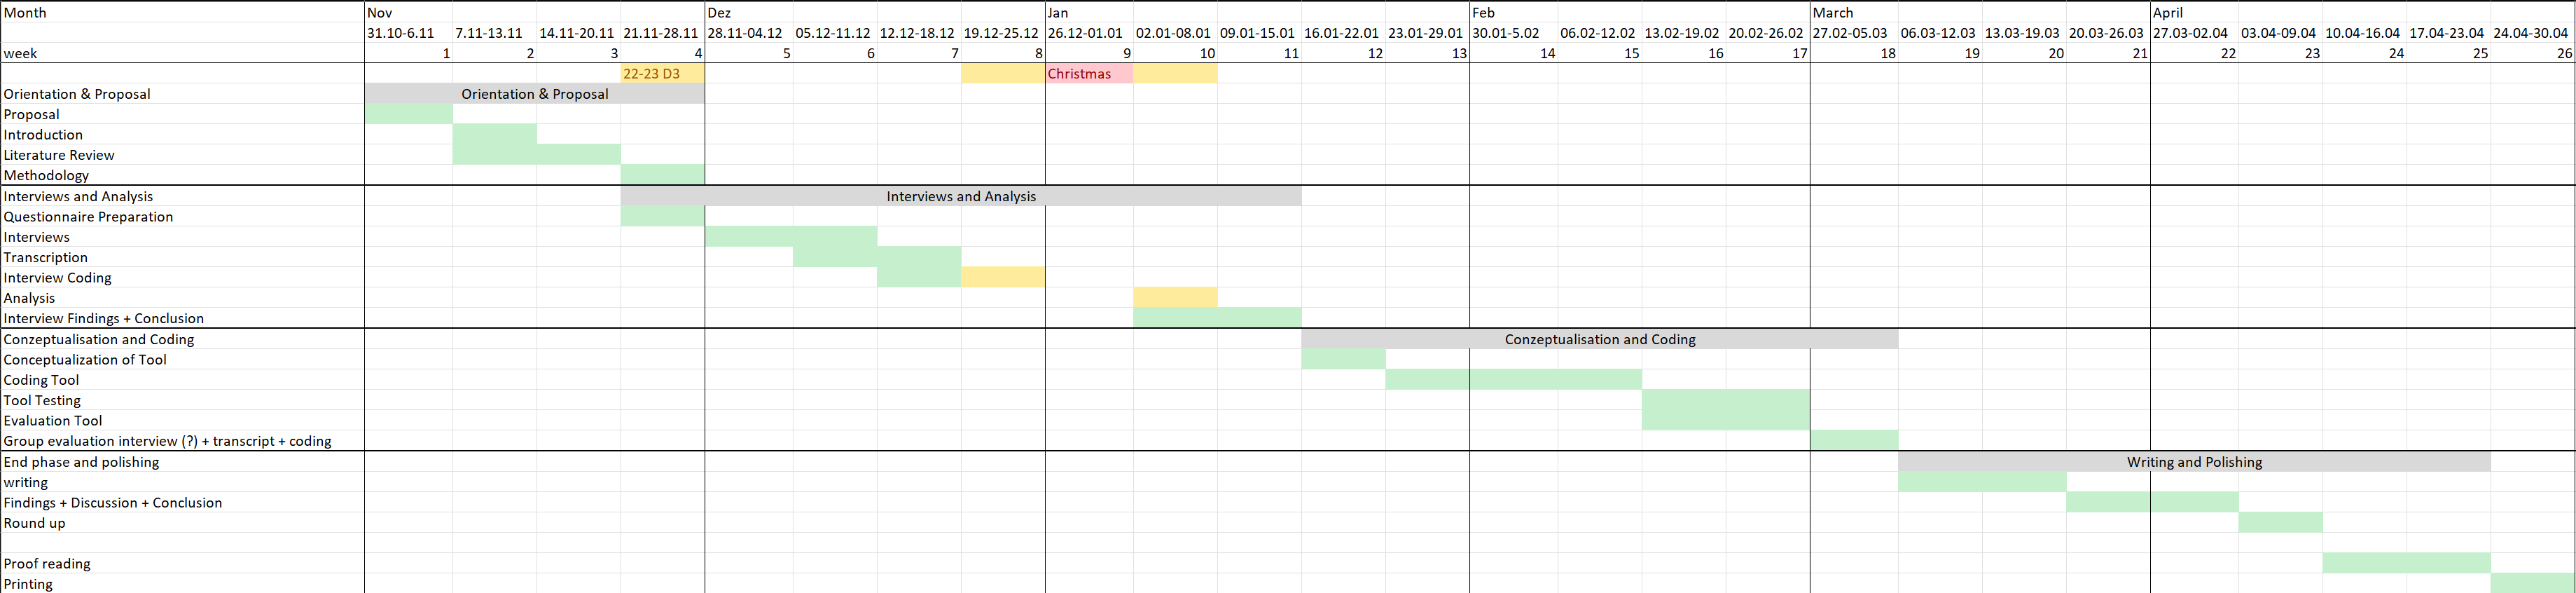
\includegraphics{Figures/SottmannBosse_timeline.png}
    \caption[Timeline Master Thesis]{Timeline Master Thesis}
    \label{fig:timeline}
    \end{figure}
    
\subsection{Outline}:
Declaration of Authorship
Abstract
Acknowledgements
Contents
List of Figures
List of Tables
List of Abbreviations

1.  Chapter: Introduction (eher ausbauen oder eher in den Literature Review Part?)
    1.1. Motivation
    1.2. General introduction and overview
    1.3. Structure
2.  Theoretical Introduction
    2.1. Case Study Area (Somalia, Somaliland, etc.)
    2.2. Project FbF and EAP (project, goal, requirements, work, context)
    2.3. Water source Monitoring – State of the Art (satellite imagery, upside, downside)
    	2.3.1. Types of Water sources
    	2.3.2. Types of transport (?)
    	2.3.3 The Case of Genders
	2.4. VGI and Crowdsensing (Ups and Downs + benefit)
    2.5. Tool and Programme introduction (overview tools, downside of tools in place, possible solution)
    2.5.1. Requirements ( based on interviews)
    2.5.2. Communication tools
    2.5.3. Data collection
    2.5.4. Data cleaning
    2.5.5. Data processing
    2.5.6. Data analysis
    2.5.7. Data Display/depiction/representation
3.  Methodology (empirical research)
    3.1. Literature/existing tools review
    3.2. Half-structured interviews
    3.2.1. With whom, how, when,
    3.2.2. About what (creation of questionnaire)
    3.2.3. Why did NYSS and other programmes not succeed?
    3.2.4. Coding + qualitative and quantitative (?) analysis
    3.2.5. Evaluation and Conclusion
    3.2.6.
    3.3. Conceptualization of a solution
    3.3.1. Synthesis Outcome Interviews + Review other Tools
    3.3.2. Structure of functioning
    3.3.3. Restructuring existing 2.7 Python Tool and Extending it
    3.3.4. Testing / Evaluation (if possible?)
4.  Results
    4.1. Literature
    4.2. Interviews
    4.3. Conceptualization
    4.4. Actual Tool
    4.5. Evaluation (?)
5.  Discussion
    5.1. Discussion methodology
    5.2. Discussion Results
    5.3. Discussion Evaluation
    5.4. Limitations
6.  Conclusion and Future outlook
7.  Eidesstattliche Erklärung
8.  References
9.  Attachements


















co-producing local and scientific knowledge is no task without challenges, data quality and continuous contributions are just two which need to be taken care of. 

To be able to integrate local knowledge
Local knowledge can be 
One way of integrating local knowledge into real-time drought monitoring is Crowdsensing


\#\#\# EAP and FbF

building on the above mentioned blocks of drought forecasts, local knowledge co-production and water source monitoring, 

\#\#\# case study (?) + current situation and general information and current tools (?)

(establish your research territory: general information about the importance, background details to understand studies context)


\#\#\# Importance of local knowledge and integration of the community

\#\#\# drought impact on local level
Why predict climate hazards if we need to understand impacts? Putting humans back into the drought equation

“There has been little effort to align the spatiotemporal granularity of socioeconomic assessments with the granularity of weather or climate monitoring.” ([Enenkel et al., 2020, p. 1161](zotero://select/groups/4773535/items/RX575C79)) ([pdf](zotero://open-pdf/groups/4773535/items/XD499UNK?page=1&annotation=QBTLFCXM))
“we highlight the need to collect and analyze environmental and socioeconomic data together and discuss novel strategies for coordinated data collection via mobile technologies from a drought risk management perspective.” ([Enenkel et al., 2020, p. 1161](zotero://select/groups/4773535/items/RX575C79)) ([pdf](zotero://open-pdf/groups/4773535/items/XD499UNK?page=1&annotation=9BUBHWNB))

“but questions related to coping capacities, migration, poverty, water supply, access to food and markets, or political conflict remain unanswered or are even decoupled from routine drought risk assessments” ([Enenkel et al., 2020, p. 1162](zotero://select/groups/4773535/items/RX575C79)) ([pdf](zotero://open-pdf/groups/4773535/items/XD499UNK?page=2&annotation=HE48ZWFA))

“The handbook of drought indicators (Svoboda et al. 2016) lists more than 50 drought indices. Not a single one of these indices connects climate anomalies to socioeconomic vulnerabilities,” ([Enenkel et al., 2020, p. 1163](zotero://select/groups/4773535/items/RX575C79)) ([pdf](zotero://open-pdf/groups/4773535/items/XD499UNK?page=3&annotation=EDKZFHJX))
--> there were more indicators in the following year, but those were limited due to availibiltiy of socioeconomic data

“In a region where migration is one of the main coping mechanisms for drought, a targeted survey focusing on the early detection of migration movements would help mobilize the timely allocation of resources by humanitarian decision-makers or even the mitigation of drought impacts.” ([Enenkel et al., 2020, p. 1167](zotero://select/groups/4773535/items/RX575C79)) ([pdf](zotero://open-pdf/groups/4773535/items/XD499UNK?page=7&annotation=N9FRDA9C))

+ humanitarian workers could focus on response rather than data acquisition (my idea)

“In addition, the impact of agricultural conditions that are not necessarily related to climate shocks, but to other factors such as pests or social conflict, could easily be monitored and used to issue early warnings and raise emergency funds before any kind of impact on crops or socioeconomic conditions is visible.” ([Enenkel et al., 2020, p. 1168](zotero://select/groups/4773535/items/RX575C79)) ([pdf](zotero://open-pdf/groups/4773535/items/XD499UNK?page=8&annotation=MDXAXIJY))

%---------------------------------------------------------
%--------------------IMPORTANT----------------------------
%---------------------------------------------------------
\todo{--> focus on water sources! Drought Indicator is good, but out of scope or at least a complete different focus}
%---------------------------------------------------------
%---------------------------------------------------------
%---------------------------------------------------------

\#\#\# value of this study
(justifying your niche - why the research is needed. -> how Gap)

\#\#\# key aims and objectives
(explain the significance of your study -> how the research was conducted -> value of the study)

Statement of objectives. Clearly and concisely, what are the general goals of the
thesis. Each thesis may have distinct goals. For instance, is your thesis project purely
descriptive of a new phenomena? Is it empirically testing causal relationships
between particular variables of interest? Adocumentclassre your providing a critical evaluation of a
particular topic or framework? Are you providing a new perspective by presenting a
new typology? Are you creating, implementing, or testing a new research tool? Any
such missions of the thesis should be clearly stated in this section.
• Significance of the project. What is the social importance of this thesis. That is, how
will this thesis aid our collective understanding of emerging media, in terms of
theory and real-world application to a particular social domain (e.g., politics, health,
entertainment, design).




The practical implementation will be based on a database and the integration of communication possibilities but could be further extended by creating visualisation and information capabilities such as a web map. On the other hand, the ability not only to receive messages but also to send messages or information to volunteers based on certain criteria, e.g. their location, could be a useful feature in the context of the uses mentioned above. Other possibilities for analysis or planning purposes, such as calculating accessibility by integrating Openrouteservice (ORS) functionality, could be future enhancements.




\#\#\# research questions and working hypothesis
(Write down at least 3 principal hypotheses that you would like to defend/verify/falsify in your thesis (it is possible that you will finally test slightly different ones during your research). You should be able to formulate hypotheses even for narrative/theoretical topics. If you have difficulties with identifying 2-3 reasonable hypotheses then your topic has no contents and you might consider changing it for somethig more reasonable.
1.	Hypothesis \#1:
2.	Hypothesis \#2:
3.	Hypothesis \#3:
4.	Other hypotheses:
)


\#\#\# outline structure


\#\#\# Methodology



1: IFRC. (n.d.). Community Engagement and Accountability. https://www.ifrc.org/community-engagement-and-accountability. [15.09.2022].
2: SRCS. (2021). Measles outbreak detected by Somaliland SRCS Volunteers in Todgheer Region. https://drive.google.com/file/d/1O9PMPKKL312o1zbXELgB7FuMdokzWpic/view. [15.09.2022].
3: SRCS (2022): Feasibility Study on Potential Use of Forecast-based Financing (FbF) for SRCS Final Report. Nottawasage Institute.
4: Start Network (2022): Integrating community voices in anticipatory action: a synthesis of complex qualitative data. Anticipatory-hub.org/news/integrating-community-voices-in-anticipatory-action-a-synthesis-of-complex-qualitative-data. [15.09.2022].

%-----------------------------------
%	SUBSECTION 1
%-----------------------------------

\subsection{Literature Review}
https://swims.faoswalim.org/livemap/view nice start! but uhh are those not up to date..

Drought
local knowledge
FbF/EAP
Red Cross/Crescent Movement

Ushahidi
CBS/NYSS
DIPAS \& SketchMapTool (as representatives for strategic data/long-term management)

%-----------------------------------
%	SUBSECTION 2
%-----------------------------------

\subsection{Proposed Methods}

Literature Review
semi-structured expert interviews: inductive approach (constructivist approach?)
6-8 categories max
address main objective + per category 2-3 follow up questions based on their answer
Introduction: Background + knowledge and expertise
Awareness: What do you know about the topic?
Location: What do you know about the country/volunteers/water sources? Specifications etc.
Topic: current drought forecasts/water source monitoring?
Pro Cons: What worked? what did not? what's about CBS or NYSS?
future outlook: what is necessary? and how?
further wishes/ideas:

tool conceptualisation



open questions: network coverage, literacy of the volunteers, educational practices/workshops
experiences with Crowdsensing?
how is the situation of water accessibility and quality?
What about gender differences?
Are there also women to talk to?


%-----------------------------------
%	SUBSECTION 3
%-----------------------------------

\subsection{Structure and Outline}

%-----------------------------------
%	SUBSECTION 4
%-----------------------------------

\subsection{Timeline}
\missingfigure{timeline}
excel sheet table

%-----------------------------------
%	SUBSECTION 5
%-----------------------------------

\subsection{Conclusion}

+ limitations and key assumptions

yeay

10\% (8 pages)

---
what is the topic of your thesis?
what are the objectives
what is the outline
methods?
thesis statement

Introduce the topic of the study.

Provide some general background info about your study.

Give a short overview of the literature review (we use the word short because the main lit review will be in Chapter Two: Literature Review.

Bring out the general idea of the study or the scope.

Provide the details of the current situation about the problem.

Describe the relevance of the research that you are going to present (note that you are introducing a study that you have already completed).

Outline the key aims and objectives of the dissertation.

Bring out the research questions or problems of the study.

Provide your hypothesis.

Outline the structure of your dissertation.

Highlight the methodology that you used to do the study.


acknowledge former studies
structure
surprise (gender and the role of "integration")
best examples and best literature review
write a draft

Motivation of the study.
Description of the study topic.
Explanation of the relevance of the study.
Explanation of the scope of the study.
Demonstration of how the study was done.
Your dissertation outline.


checklist:
Does the proposal have imagination?
Is the problem stated clearly?
(a) hypothesis clear? testable?
(b) if no hypothesis, are objectives clearly stated? Can they be accomplished?
(c) problem perhaps too large?
Is the methodology feasible?
(a) can data be collected?
(b) how will data be analyzed?
(c) will the analysis allow the acceptance or rejection of the hypothesis?
(d) is the sample population overused?
What might the results of the analysis look like? (tables, graphs, etc.)
What are the consequences if
(a) the experiment fails;
(b) data cannot be obtained;
(c) analysis is inconclusive;
(d) hypothesis is rejected or accepted?
Can major research activities be listed?
Can a time estimate be made for each activity?
Again, are the dimensions of the project manageable?

\todototoc
\listoftodos